\section{NP Completeness}
\begin{itemize}
	\item Let's revisit the independent set problem. Earlier we did this on trees, but now we're going to 
		move to a general graphs.
	\item Given a graph \( G = (V, E) \) with \( n \) vertices and \( m \) edges, along with an integer 
		\( 1 \le  k \le n \)
	\item We want to return an independent set of size \( k \). 
	\item A naive algorithm for this problem is to just try all sets of \( k \) vertices. This takes 
	\( O{n \choose k} \in \Omega(n^k) \) 
	\item This is good if \( k \) is small, but gets significantly worse as \( k \) gets large, say 
		\( k = n / 2 \). In this case, then the algorithm runs in approximately \( O(n^n) \) time.  
	\item In the real world, what we try to show is that this is an NP-hard problem -- in other words, we should 
		stop trying to look for an efficient solution.
		\begin{itemize}
			\item The approach hinges on the fact that problems in NP-hard are not believed to have efficient 
				solution algorithms, so we should stop trying basically.
			\item By showing that a problem is NP-hard, it also shows that it's NP-complete.

				\question{Is this because every NP-complete problem reduces to a NP-hard problem?}
		\end{itemize}
	\item Our approach to showing that a problem is NP-hard is to show that a well known NP-complete problem 
		reduces to our problem of interest. 
	\item Recall our tree of problems from last lecture:
		\begin{center}
			\begin{tikzpicture}[every text node part/.style={align=center}]
				\foreach \x in {0, 4}
						\draw[-stealth] (\x+0.5, 0) -- (\x+2, 0);
				\draw node at (-1, 0) {Every problem \\ in NP};
				\draw node at (3.25, 0) {Circuit\\SAT};
				\draw node at (7.25, 0) {3-SAT};
				\draw [-stealth] (8, 0) -- (10, 1.5) node[right] {Independent \\ Set};
				\draw [-stealth] (8, -0.2) -- (10, -1.5) node[right] {Rudrata Cycle};
			\end{tikzpicture}
		\end{center}
		And also recall our approach to showing NP-completeness:
		\begin{enumerate}[label=\arabic*.]
			\item We first show that \( A \in \text{NP} \). 
			\item We show NP-completeness by showing that an NP-complete problem  \( B \) reduces to \( A \). 
		\end{enumerate}
		By doing this, we show that a polynomial algorithm that solves \( A \) will also solve \( B \).
\end{itemize}
\subsection{NP-hardness of Independent Set}
\begin{itemize}
	\item We want to choose an NP complete problem to reduce to independent set. Here, we'll choose the 3-sat
		problem.
		
		\question{Are all NP-hard problems also NP-complete?}
	\item Recall the 3-sat problem, where we're given an instance \( \psi \) :
		\begin{align*}
			(x \lor y \lor z) \land (\overline z \lor \overline w \lor x) \land (y \lor \overline z \lor w)
		\end{align*}
		and we want to find an assignment for \( x,y,z,w \) such that this instance returns true.  
	\item To show reduction to independent set, we go to each clause and make a ``subgraph'' consisting 
		of the variables in the clause. We do this for all three clauses:
		\begin{center}
			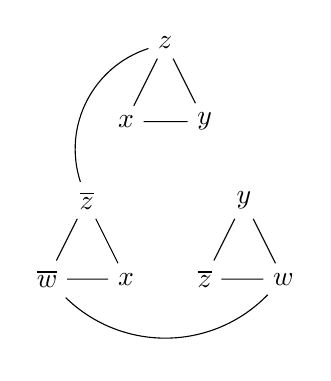
\begin{tikzpicture}
				\draw node (x1) at (-0.5, 0) {\( x \) };
				\draw node (y1) at (0.5, 0) {\( y \) };
				\draw node (z1) at (0, 1) {\( z \) };
				\draw (x1) -- (y1) -- (z1) -- (x1);

				\draw node (wbar2) at (-1.5, -2)  {\(  \overline w \) };
				\draw node (x2) at (-0.5, -2) {\( x \) };
				\draw node (zbar2) at (-1, -1) {\( \overline z \) };
				\draw (zbar2) -- (x2) -- (wbar2) -- (zbar2);

				\draw node (y3) at (1, -1) {\( y \) };
				\draw node (zbar3) at (0.5, -2) {\( \overline z \) };
				\draw node (w3) at (1.5, -2) {\( w \) };
				\draw (y3) -- (zbar3) -- (w3) -- (y3);
				\draw[out= -45, in = -135, relative] (wbar2) to (w3);
				\draw[out= -45, in = -135, relative] (z1) to (zbar2);
			\end{tikzpicture}
		\end{center}
	\item Note that in our graph, we don't connect the two \( y \) 's that appear, since they are part of 
		different clauses.
	\item For the variables that are set to 1, this corresponds to selecting that vertex for our independent 
		set instance. 
	\item For all variables that contain the literal and its negation, we should also connect an edge between 
		those because we want only one of \( x \) and \( \overline x \) to be selected. 
	\item Note that for every set of 3 vertices, we can only select one of the three vertices in order for the 
		clause to remain independent.  
	\item This also suggests our polynomial-time recovery algorithm: whenever \( x \) is chosen in the independent
		set, then set \( x  =1\). If \( \overline x \) appears, then set \( x = 0 \). If it doesn't appear at 
		all, then we don't care what it's set to. 
\end{itemize}
\subsubsection{Formal Proof of Reduction}
\begin{itemize}
	\item There's always two parts these kinds of proofs: we have to show that the reduction algorithm works, and also 
		that the recovery algorithm works.
	\item For the first part: we want to show that if the 3-sat instance \( \psi \) has a satisfying assignment 
		\( A: \{x_1, \dots, x_n\} \to \{0, 1\}  \), then graph \( G \) has an independent 
		set instance \( I \) of size \( k = m \). 
		\begin{itemize}
			\item For each clause \( x_i \lor \overline {x_j} \lor x_\ell \), we know that \( A \) sets one of 
				\( x_i, \overline x_j, x_\ell \) to 1.
			\item WLOG choose \( x_i \). Now, we'll add node \( x_i \) to the independent set. 
			\item This means that our instance \( I \) is indeed of size \( m = k \). 

				\question{why is this true?}

				\answer{because \( k \) is the number of clauses, and we have to set one of these to 1 
				for every clause!}
			\item We know that our selection rules state that we never select both \( x_i \) and 
				\( \overline {x_i} \), so therefore we guarantee that our set is independent.
		\end{itemize}
	\item Now for part 2: Let \( I  \) be an independent set in  \( G \) of size \( k \). We show that the 
		recovery algorithm outputs a satisfying assignment.
		
		Recall that our recovery algorithm has variables \( x_i \), and it sets \( x_i = 1 \) if 
		\( x_i \in I \), and \( x_i = 0 \) if \( \overline {x_i} \in I\). 
		\begin{itemize}
			\item For each \( i \), our recovery algorithm either finds \( x_i \) or \( \overline {x_i} \) (and 
				never both), so 
				our recovery algorithm is well defined.
			\item Further, based on the way that we constructed our graph, only one of the nodes in any 
				subgraph will be selected, meaning that it makes that particular clause return true. Therefore, 
				we do output a satisfying instance.
		\end{itemize}
\end{itemize}
\subsection{Clique}
\begin{itemize}
	\item Here, we're given a graph \( G \) and an integer \( 1 \le  k \le n \), and we want to output a
		clique of size \( k \). 
	\item To show that this problem is also NP-hard, we show that independent set reduces to Clique. 
		\begin{itemize}
			\item To reduce, we ``invert'' the graph by creating a graph \( \overline G \), which contains 
				the same vertices \( v \) but the edges not in \( G \). Then, if we can 
				find an independent set on \( \overline G \), then we know that in the original graph \( G \) 
				it must be a clique. 
			\item The recovery algorithm is basically the same thing but in reverse: we just return the vertices
				found in the independent set. 
		\end{itemize}
\end{itemize}
\subsection{Rudrata (s, t)-path}
\begin{itemize}
	\item Given a graph \( G = (V, E) \) and vertices \( s, t \), we want to find a path starting at \( s \), 
		end at \( t \), while also visiting each vertex exactly once. 
	\item Here, we're going to show that this problem reduces to another NP-complete problem, instead of the 
		other way around. Specifically, we're going to show that this reduces to the Rudrata cycle problem. 
		
		\comment{We're doing this only as an example to further show reduction, this does not have anything to do 
		with proving hardness}
	\item \textit{Proof:} Given a Rudrata \( (s, t) \)-path instance, we can generate a reduction algorithm
		 as follows:
		
		 \question{Review this later}
\end{itemize}
\subsection{Double Cycle}
\begin{itemize}
	\item Given a graph \( G = (V, E) \) with \( n \) vertices, with the restriction that \( n \) is even.
	\item We want to find two disjoint cycles of size \( n / 2 \) vertices, which will visit each node exactly 
		once. 
	\item Again, we will show that this reduces to rudrata cycle.
\end{itemize}
